\section{Individual Fairness}
\textbf{DEF:} A model $M$ is individually fair if for any similar $x,x'$ it produces similar outputs $M(x),M(x')$, e.g.
\begin{itemize}
    \item Lipschitz continuity: $\mu(M(x),M(x'))\le L\phi(x,x')$.
    \item Binary similarity: $\phi(x,x')\Rightarrow M(x)=M(x')$.
\end{itemize}
% Then use DL2 to translate the similarity constraint into loss functions.

\subsection*{Fair Representation Learning:}
\begin{itemize}
    \item Data Regulator: Determines fairness criteria and data source(s), audits results.
    \item Data Producer: Computes the fair representation given data regulator criteria.
    \item Data Consumer: Trains the ML model given the sanitized data.
          Split models into an encoder $f_\theta$ (data producer) and a predictor $h_\psi$ (data consumer).
\end{itemize}

\subsection*{LCIFR}
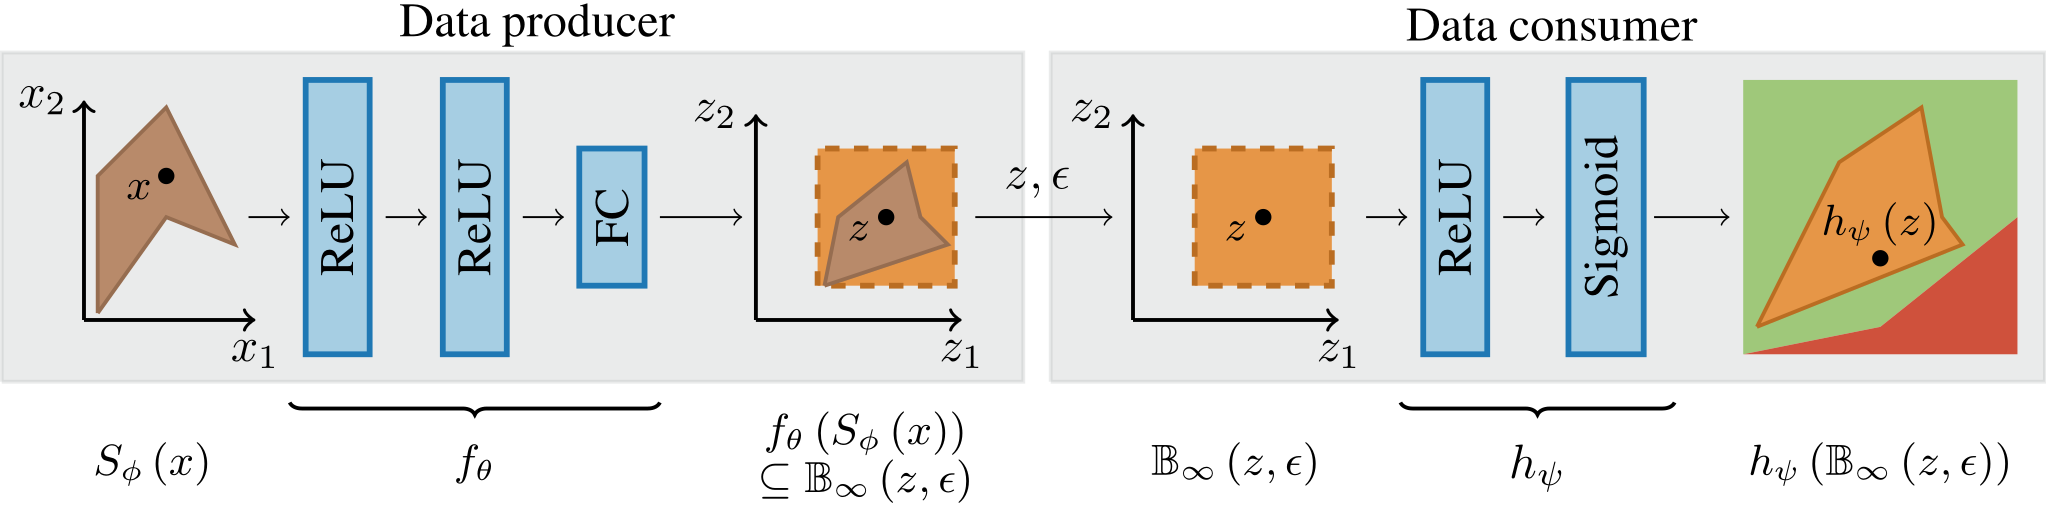
\includegraphics[width=1\columnwidth]{img/lcifr.png}
Consider binary $\phi,\mu$. 1. Encoder $f_\theta$ is trained s.t. $\phi(x, x') \Rightarrow \|f(x) - f(x')\|_\infty \leq \delta$ (with a combined loss ensuring informativeness of the representations) using DL2 (or $\delta$ is computed when encoded as MILP). 2. Use $L_\infty$-robustness training on encoded data for perturbations of magnitude $\delta$ and certify robustness. Gives certified individual fairness. Problem: Relies on NN verifiers so not scalable to real-world models.

\subsection*{LASSI}
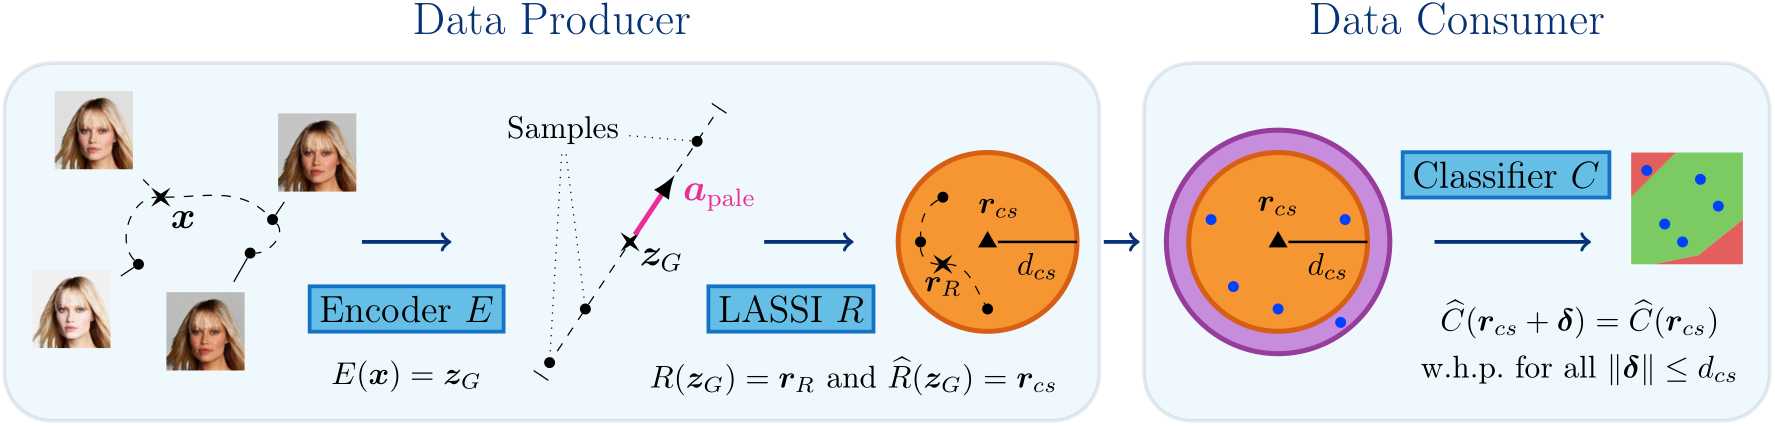
\includegraphics[width=1\columnwidth]{img/lassi.png}
1. Data producer uses center smoothing to get an encoder that provably maps all similar points close together with high probability. 2. Data consumer uses randomized smoothing to certify that all points within a certain radius get classified the same with high probability. Problem: Depends on quality of generative model.

\section{Group Fairness}
\textbf{Demographic Parity}\\
$\P\left[\hat Y\mid G=0\right]=\P\left[\hat Y\mid G=1\right]$\\
\textbf{Equalized Odds}\\
$\P\left[\hat Y\mid G=0,Y=0\right]=\P\left[\hat Y\mid G=1,Y=0\right]$\\
$\P\left[\hat Y\mid G=0,Y=1\right]=\P\left[\hat Y\mid G=1,Y=1\right]$\\
\textbf{Equal Opportunity}\\
$\P\left[\hat Y\mid G=0,Y=1\right]=\P\left[\hat Y\mid G=1,Y=1\right]$

\textbf{Approaches:}
\begin{itemize}
    \item Pre-processing: Debias the data, such that standard training yields a fair model. E.g. fair representation learning.
    \item In-training: Change the training pipeline to learn a fair model (on biased data). E.g. add soft fairness constraint to the loss.
    \item Post-processing: Modify predictions at inference time. E.g. different thresholds for different groups.
\end{itemize}

\subsection*{LAFTR}
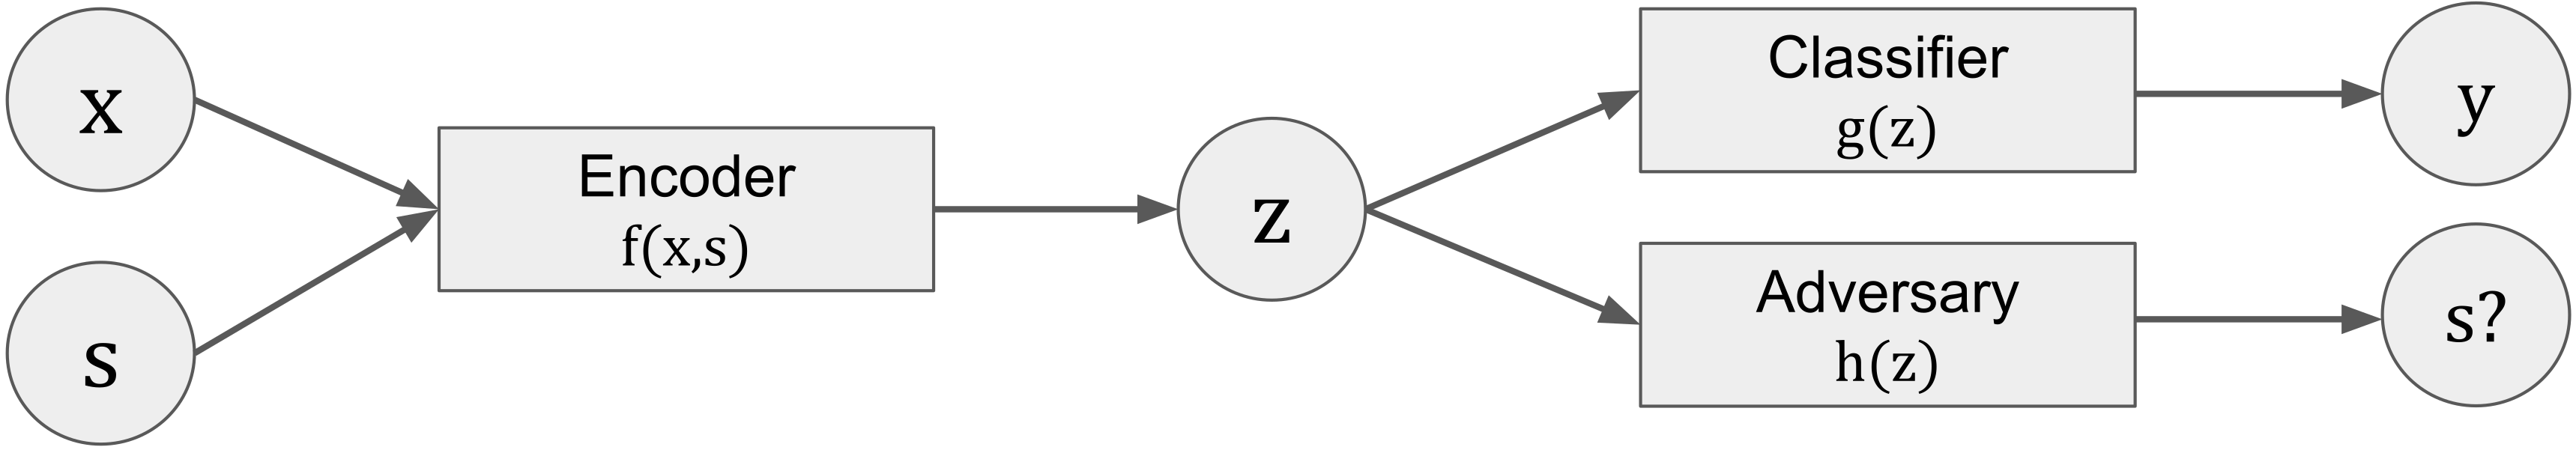
\includegraphics[width=1\columnwidth]{img/laftr.png}
Jointly trains an encoder $f$, classifier $g$, and adversarial classifiers $h$ by solving\\
$\min_{f,g}\max_{h\in\mathcal{H}} \mathcal{L}_{\text{clf}}(f,g)-\lambda \mathcal{L}_{\text{adv}}(f,h)$.\\
\textbf{Balanced Accuracy}\\
$\operatorname{BA}(h)=\frac{1}{2}\E_{Z_0}\left[1-h(z)\right]+\frac{1}{2}\E_{Z_1}h(z)$\\
$h^*=\argmax_h\operatorname{BA}_{Z_0,Z_1}(h)=\mathbbm{1}_{\{p_1(z)\geq p_o(z)\}}$\\
% % \vfill\null
% \columnbreak
\textbf{DP-Distance} (Relaxation of DP)\\
$\Delta^{\text{DP}}_{Z_0,Z_1}(g)=\left|\E_{Z_0}g(z)-\E_{Z_1}g(z)\right|$\\
$\Delta^{\text{DP}}_{Z_0,Z_1}(g)\leq2\operatorname{BA}_{Z_0,Z_1}(h^*)-1$\\
LAFTR estimates $\Delta^{\text{DP}}_{Z_0,Z_1}(g)$ given an adversary $h$. Fairness is overestimated (there may be better adversaries).

\subsection*{Fair Normalizing Flows}
Normalizing flows for a distribution $p(z)$ parameterize $z=f(x)$ where $x$ is sampled from a simple distribution $q(x)$ through an invertible transformation: $p(z)=q(f^{-1}(z))\left|\det{\partial_z f^{-1}}(z)\right|.$\\
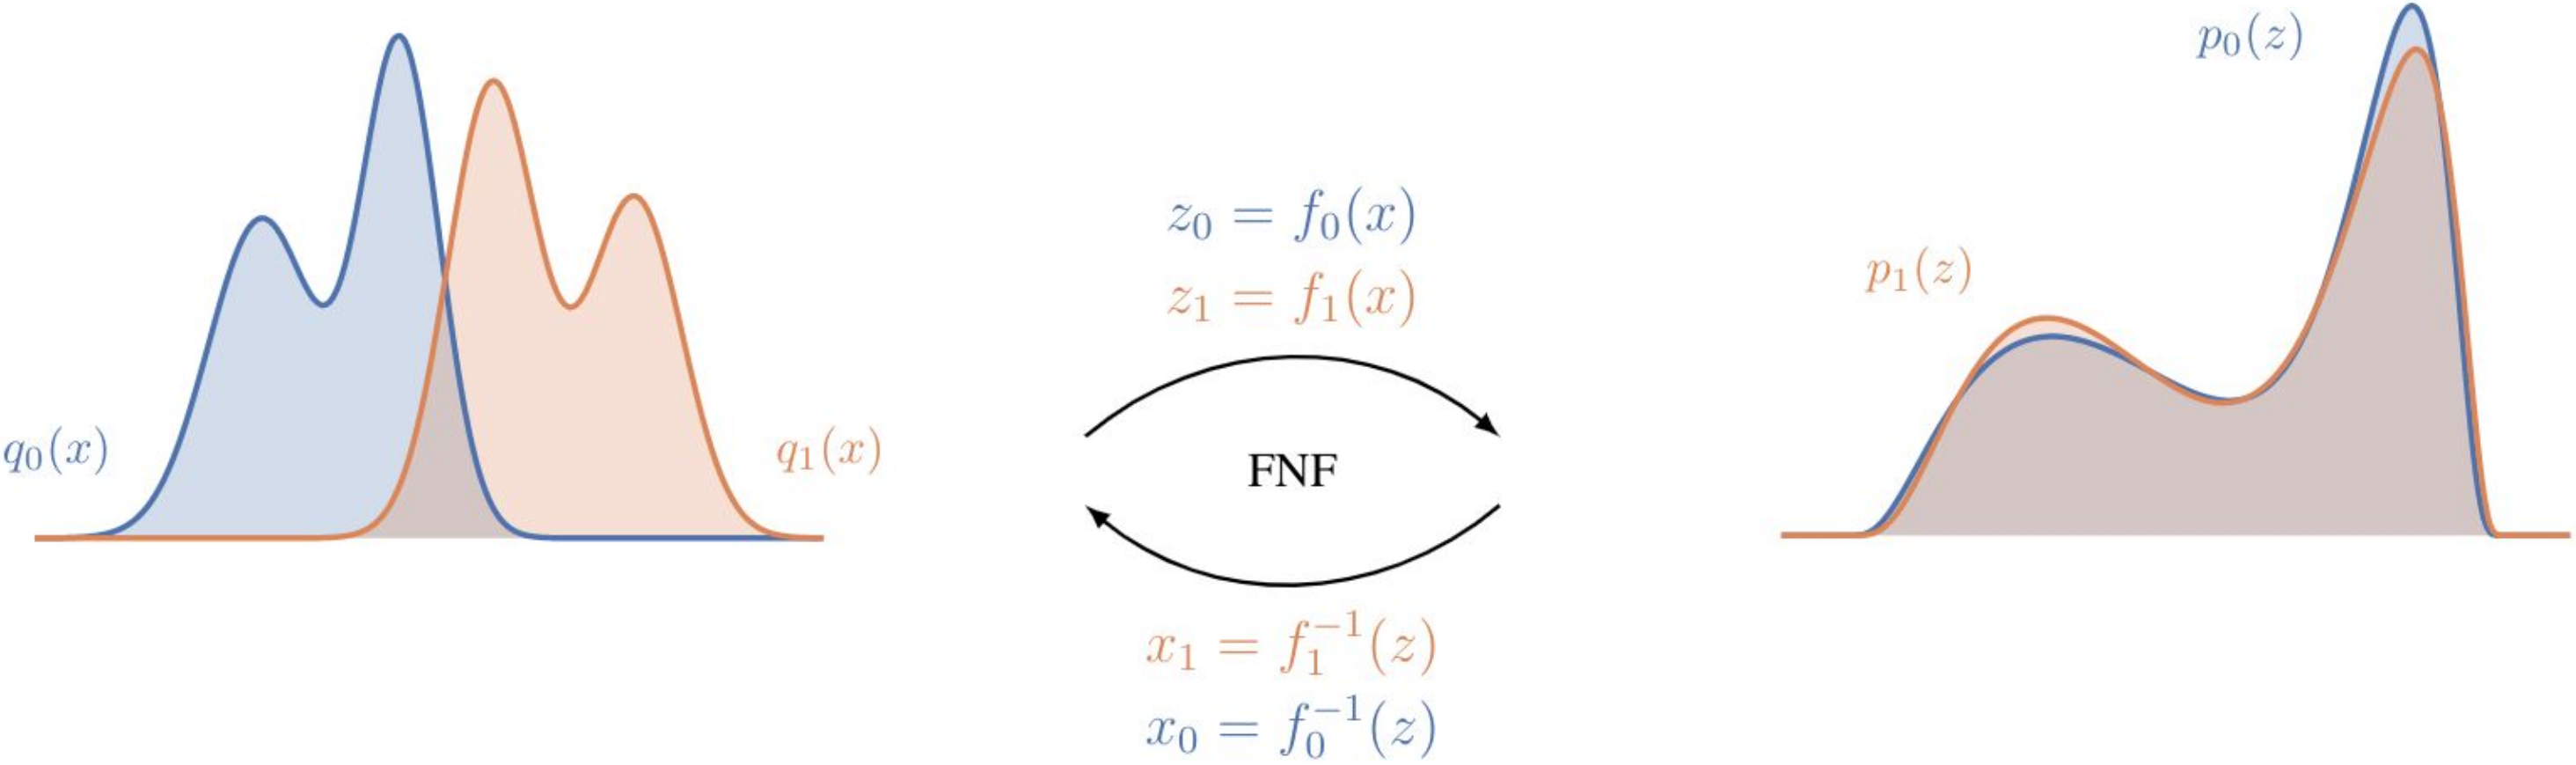
\includegraphics[width=1\columnwidth]{img/fnf.png}
FNF learns two flows $f_0,f_1$ as encoders for $Z_0,Z_1$. 1. Estimate densities $q_0, q_1$ for both groups. 2. Apply the encoder to get $z=f_0(x)$ (or $f_1(x)$), and use the flows and $q_0,q_1$ to get $p_0(z)$ and $p_1(z)$. 3. Use $p_0(z)$ and $p_1(z)$ to estimate the optimal adversary $h*$ and then upper bound its balanced accuracy with probability $1-\varepsilon$ (Hoeffding) 4. Use the inequality from LAFTR above to upper bound the DP-distance of any downstream classifier trained on representations z with probability $1-\varepsilon$.

To get tight bounds: train the flows to promote low accuracy of $h^*$ by minimizing $D_{KL}(p_0||p_1)+D_{KL}(p_1||p_0)$. \Warning The guarantees hold for the estimated $q_0,q_1$.

\subsection*{FARE}
Restrict representations $z$ to a finite set. This allows bounding $\operatorname{BA}_{Z_0,Z_1}(h^*)$ whp. directly. Use fairness-aware decision tree as encoder which is obtained by training a tree to have unbalanced leaves wrt. $y$ and uniform leaves wrt. $s$. Gives provable unfairness upper bound with no restrictive assumptions